\documentclass[11pt,letterpaper]{article}
\usepackage{graphicx, geometry, amsmath, hyperref, url, natbib, booktabs, xcolor, listings, tabularx}
\geometry{margin=1in}
\hypersetup{colorlinks=true, linkcolor=black, citecolor=black, urlcolor=black}
\makeatletter
\g@addto@macro{\UrlBreaks}{\UrlOrds}
\makeatother

\title{Host vocabulary predicts whether new scientific concepts take root across disciplinary boundaries}
\author{}
\date{}

\begin{document}
\maketitle

\begin{abstract}
When a scientific concept first appears in a new disciplinary subfield, what determines whether it takes root?
We study 426 emerging concepts and 462,812 works from OpenAlex across physics, computer science and biomedicine.
The unit of analysis is a host-entry event: the first year a concept appears in a non-origin subfield together
with at least five co-occurring partner terms. We measure the host-vocabulary share of these partners and test
whether it predicts uptake by newcomer authors over the following five years. On an independent MeSH biomedical
population, a one-standard-deviation increase in host-vocabulary share raises newcomer uptake by 23\%
(pre-registered and replicated; incidence-rate ratio 1.23, 95\% CI 1.12 to 1.36). Development-set estimates on
the main-arm folds are concordant. The strict fixed-effects specification is inconclusive on the Held-out fold
(IRR 0.98, 95\% CI 0.70--1.37, 30 clusters). At the adopter level, authors who take up a concept
are enriched for prior exposure to its entry partners (OR 3.09; prevalence 0.79 vs.\ 0.61).
Co-transfer of origin companions is null. The population is dominated by
physics and computer-science concepts from arXiv; generalisation to social sciences and humanities is untested.
\end{abstract}

\noindent\textbf{Keywords:} Knowledge diffusion, emerging concepts, co-word network, host vocabulary,
cross-disciplinary integration, applied network science, scientometrics, concept emergence.

\section{Background}
\label{sec:background}

Scientific knowledge advances through discoveries within disciplinary boundaries and through the
migration of concepts, methods and results across them~\citep{Uzzi2013, Wang2017}. Yet most new ideas that appear
outside their field of origin fail to establish a lasting presence. What distinguishes the entries that take root
from those that fade?

Prior work has examined this question from several angles. \citet{Cheng2023} showed that a concept's fit with
existing intellectual traditions, measured as mean cosine similarity of neighbour terms in a global word-embedding
space, predicts its annual article count. \citet{Deichmann2020} found that connectivity within the existing
knowledge network shapes how far an idea diffuses. \citet{Boschma2014} demonstrated at the city level that
technological diversification is path-dependent: regions branch into technologies related to their existing
portfolio. In network science, studies of co-word dynamics have traced the structural signatures of emerging
topics~\citep{Chen2009} and the roles of bridging and brokerage~\citep{Burt2004, Guimera2005}.
\citet{Chavalarias2013} introduced phylomemetic networks for reconstructing the dynamics of science,
modelling lineage relationships between scientific fields from large-scale co-word data.
\citet{Salatino2017} studied how topics are born by analysing the research dynamics preceding
the emergence of new areas. \citet{Salatino2018augur} used these dynamics to forecast emerging topics,
finding that new areas tend to arise at the intersection of weakly connected parent communities.
These studies treat connectivity or semantic similarity as global properties of a concept. None of them measures
the host-specific vocabulary composition of the very first papers that carry a concept into a new subfield, nor
tests whether this entry-level composition predicts durable adoption.

We address two research questions (Figure~\ref{fig:overview}). RQ1 (emergence precursors) asks which structural
patterns in an evolving co-word network characterise concept emergence. RQ2 (cross-disciplinary diffusion) asks
how concepts spread across disciplinary communities, and specifically whether host-vocabulary composition at the
moment of entry predicts later uptake. RQ2 is the paper's primary contribution. RQ1 provides the network context
and tests a complementary hypothesis about pre-emergence openness.

Our main finding is that when a concept enters a new host subfield, the share of its entry partners that belong
to the host's vocabulary predicts uptake by newcomer authors over the following five years. We call this the
\emph{host-entry grafting} effect. It replicates on an independent MeSH biomedical population (co-primary
IRR 1.23, 95\% CI 1.12 to 1.36; verdict: REPLICATED), with concordant development-set estimates on the
main-arm folds (Screen co-primary IRR 1.30; Held-out co-primary IRR 1.19, 95\% CI 1.06 to 1.33; both folds
were used in pipeline development and are not true held-out tests). The effect is host-specific rather than a
proxy for general concept accessibility, though the latter test is limited by near-collinearity between the
Balassa-index lift measure and the continuous host-vocabulary share. Co-transfer of origin companions, defined
as the fraction of entry partners that were prior companions in the concept's origin field, is null in all
specifications. A complementary structural finding is that emerging concepts show lower persistent-neighbour
closure, defined as the closure coefficient restricted to top associates present in consecutive years, before
sustained uptake. On the Held-out fold, the panel coefficient for persistent-neighbour closure is $-1.07$
(Holm $p = 0.015$); the matched event-study standardised mean difference on the same fold is $-0.83$
(95\% CI $[-1.71, -0.10]$). Both are development-set estimates, and the general closure measure fails
(Holm $p = 0.147$).

\paragraph{Contributions.}
\begin{enumerate}
\item A pre-registered host-entry test showing that the host-vocabulary composition of a concept's initial
partners predicts newcomer uptake, replicated on an independent MeSH biomedical population (co-primary
IRR 1.23, 95\% CI 1.12 to 1.36, verdict REPLICATED; development-set estimates concordant: Screen IRR 1.30,
Held-out IRR 1.19).%
\footnote{Code:
\url{https://github.com/ai-inventor-papers/ai-invention-8892b7-occupancy-is-not-integration-for-new/tree/fork/run_desxWCcMY1R1/round-3/experiment-7},
\url{https://github.com/ai-inventor-papers/ai-invention-8892b7-occupancy-is-not-integration-for-new/tree/fork/run_desxWCcMY1R1/round-4/evaluation-2},
\url{https://github.com/ai-inventor-papers/ai-invention-8892b7-occupancy-is-not-integration-for-new/tree/fork/run_desxWCcMY1R1/round-4/experiment-9}.}
(Section~\ref{sec:rq2_results}).

\item A semantically grounded, outcome-blind dataset of 426 emerging concepts with 462,812 OpenAlex works
and an independent 191-concept MeSH biomedical check population.%
\footnote{Code:
\url{https://github.com/ai-inventor-papers/ai-invention-8892b7-occupancy-is-not-integration-for-new/tree/fork/run_desxWCcMY1R1/round-2/dataset-5},
\url{https://github.com/ai-inventor-papers/ai-invention-8892b7-occupancy-is-not-integration-for-new/tree/fork/run_desxWCcMY1R1/round-1/dataset-3}.}
(Section~\ref{sec:data}).

\item Evidence that the host-vocabulary effect is host-specific (though the Balassa-index lift leg of this
test is near-collinear with the continuous share) and operates through both the extensive margin (whether
uptake starts) and the intensive margin (its magnitude), with no detectable variation by origin field.%
\footnote{Code:
\url{https://github.com/ai-inventor-papers/ai-invention-8892b7-occupancy-is-not-integration-for-new/tree/fork/run_desxWCcMY1R1/round-5/evaluation-6},
\url{https://github.com/ai-inventor-papers/ai-invention-8892b7-occupancy-is-not-integration-for-new/tree/fork/run_desxWCcMY1R1/round-5/evaluation-7}.}
(Section~\ref{sec:rq2_mechanism}).

\item A pre-registered test of structural precursors of emergence finding that general closure fails on the
Held-out fold while the panel coefficient for persistent-neighbour closure is significant ($-1.07$,
Holm $p = 0.015$; development-set estimate), and that the effect is not Burt brokerage.%
\footnote{Code:
\url{https://github.com/ai-inventor-papers/ai-invention-8892b7-occupancy-is-not-integration-for-new/tree/fork/run_desxWCcMY1R1/round-3/experiment-5},
\url{https://github.com/ai-inventor-papers/ai-invention-8892b7-occupancy-is-not-integration-for-new/tree/fork/run_desxWCcMY1R1/round-4/evaluation-3}.}
(Section~\ref{sec:rq1_results}).

\item A stable two-type diffusion typology, an expansion-before-diffusion ordering, adopter-level enrichment
for prior partner exposure, and four representative cases.%
\footnote{Code:
\url{https://github.com/ai-inventor-papers/ai-invention-8892b7-occupancy-is-not-integration-for-new/tree/fork/run_desxWCcMY1R1/round-3/experiment-8},
\url{https://github.com/ai-inventor-papers/ai-invention-8892b7-occupancy-is-not-integration-for-new/tree/fork/run_desxWCcMY1R1/round-4/evaluation-4},
\url{https://github.com/ai-inventor-papers/ai-invention-8892b7-occupancy-is-not-integration-for-new/tree/fork/run_desxWCcMY1R1/round-4/evaluation-5}.}
(Sections~\ref{sec:rq2_typology} and~\ref{sec:rq2_adopter}).
\end{enumerate}

\begin{figure}[!htbp]
  \centering
  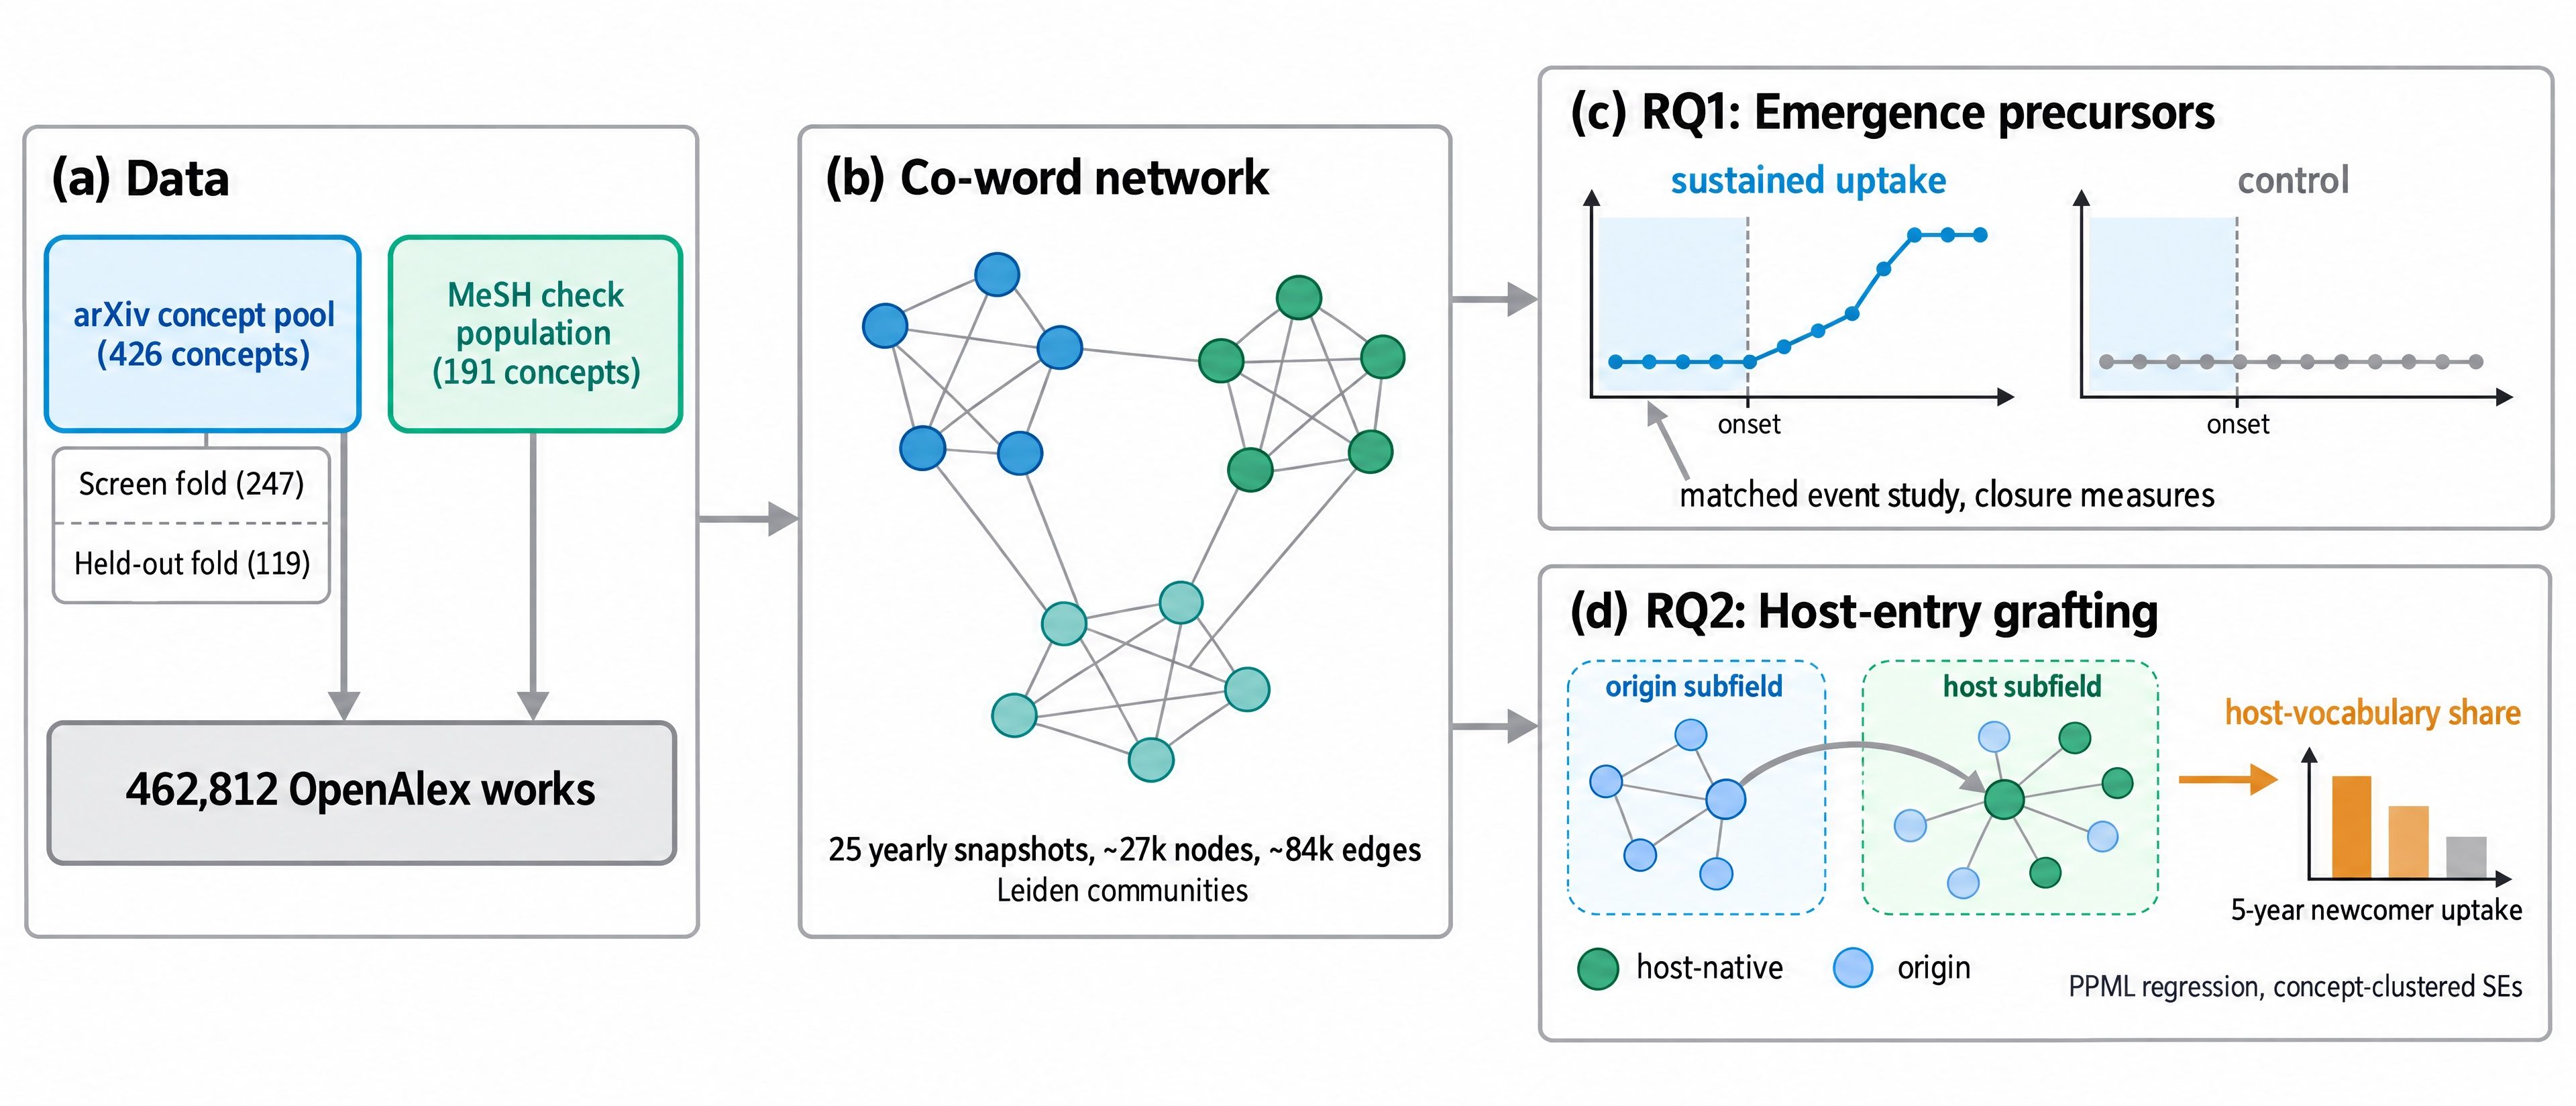
\includegraphics[width=\linewidth,height=0.85\textheight,keepaspectratio]{figures/fig1_v0.jpg}
  \caption{Overview of the study design. (a)~Data: an outcome-blind arXiv concept pool of 426 emerging
  scientific concepts, split into a screen fold (247) and a held-out fold (119), and an independent MeSH
  biomedical check population of 191 concepts. Both are drawn from 462,812 OpenAlex works. (b)~Co-word
  network: yearly co-word snapshots (25 snapshots, ${\sim}$27k nodes, ${\sim}$84k edges) with Leiden
  communities; the schematic shows three colour-coded communities. (c)~RQ1, emergence precursors: a matched
  event study compares closure measures in the pre-onset window (shaded) between concepts showing sustained
  uptake (blue, rising after onset) and controls (grey, flat). (d)~RQ2, host-entry grafting: a concept enters
  a non-origin host subfield (light blue $\rightarrow$ light green region). Its partner terms are either
  host-native (dark green) or from the origin vocabulary (light blue). The host-vocabulary share (orange) is
  the exposure in a pre-registered PPML regression with concept-clustered standard errors predicting 5-year
  newcomer uptake. The timelines and bars in (c) and (d) are schematic and carry no data values.}
  \label{fig:overview}
\end{figure}

\section{Methods}
\label{sec:methods}

The study proceeds in four stages, corresponding to the panels of Figure~\ref{fig:overview}.
First, we assemble an outcome-blind concept pool and a co-word network from OpenAlex
(panel~a, Section~\ref{sec:data}). Second, we build yearly co-word snapshots with Leiden
communities and identify structural precursors of emergence through a matched event study
(panel~b and~c, Section~\ref{sec:rq1method}). Third, we define host-entry events, measure
the host-vocabulary share of each event's co-occurring partners, and test whether this share
predicts five-year newcomer uptake in a pre-registered PPML regression
(panel~d, Section~\ref{sec:rq2method}). Fourth, we decompose the effect into extensive and
intensive margins, test host-specificity, and examine adopter-level mechanisms
(Section~\ref{sec:decomposition}).

\subsection{Data}
\label{sec:data}

\paragraph{Concept pool.} We assembled an outcome-blind pool of 426 emerging scientific concepts, where
outcome-blind means that the inclusion criteria and frame were frozen and SHA-256-hashed before any
post-appearance data were inspected. Concepts are noun-phrase surface forms that first appeared in
OpenAlex~\citep{Priem2022} titles and abstracts between 2005 and 2016, with 20 to 300 papers in the
first-appearance window and no more than 8,000 total works through 2024.%
\footnote{Code: \url{https://github.com/ai-inventor-papers/ai-invention-8892b7-occupancy-is-not-integration-for-new/tree/fork/run_desxWCcMY1R1/round-1/dataset-1}.}
Of the 426, 366 are main emerging concepts (247 Screen, 119 Held-out, split by a SHA-1 hash on concept
identifiers) and 60 are stationary reference concepts. A logistic-regression classifier trained on
silver-standard labels (F1 $= 0.82$ on 300 test items, AUC $= 0.89$) and a variant merger (B-cubed
F1 $= 0.78$) were applied to ground every concept.%
\footnote{Code: \url{https://github.com/ai-inventor-papers/ai-invention-8892b7-occupancy-is-not-integration-for-new/tree/fork/run_desxWCcMY1R1/round-2/experiment-1}.}
The pool is dominated by physics, physical-sciences and computer-science concepts sourced from arXiv.
For the Screen fold, 202 concepts survive grounding filters; for the Held-out fold, 100.

\paragraph{MeSH check population.} An independent biomedical arm of 191 concepts was drawn from new MeSH
descriptors (DateEstablished 2006 to 2016, widened to 2004--2005 and 2017--2018), surviving a provenance
filter, a PubMed novelty pre-screen and the same early-volume rule. Only approximately 25\% of new MeSH
descriptors are genuinely new concepts; the remainder are reclassifications or splits.

\paragraph{Works.} The combined corpus comprises 462,812 unique OpenAlex works with 488,078 verified
concept--work links, spanning 2000 to 2024.

\paragraph{Co-word network.} From a design-weighted whole-science background sample of 259,716 works, we
built 25 yearly three-year-window co-occurrence snapshots (approximately 27,000 nodes and 84,000 edges per
snapshot), with association-strength edge weights~\citep{vanEck2009}, Leiden community
detection~\citep{Traag2018} (best of five seeds) and alluvial community identifiers.%
\footnote{Code: \url{https://github.com/ai-inventor-papers/ai-invention-8892b7-occupancy-is-not-integration-for-new/tree/fork/run_desxWCcMY1R1/round-2/experiment-3}.}

\paragraph{Host-nativeness profiles.} For each concept-keyword node, we retrieved exact OpenAlex
subfield-by-time-block publication counts, covering 78.7\% of host co-occurrence weight across 1,372 nodes.
These profiles supply the host-vocabulary share used in RQ2. Figure~\ref{fig:network} shows a schematic of the
resulting network.

\begin{figure}[!htbp]
  \centering
  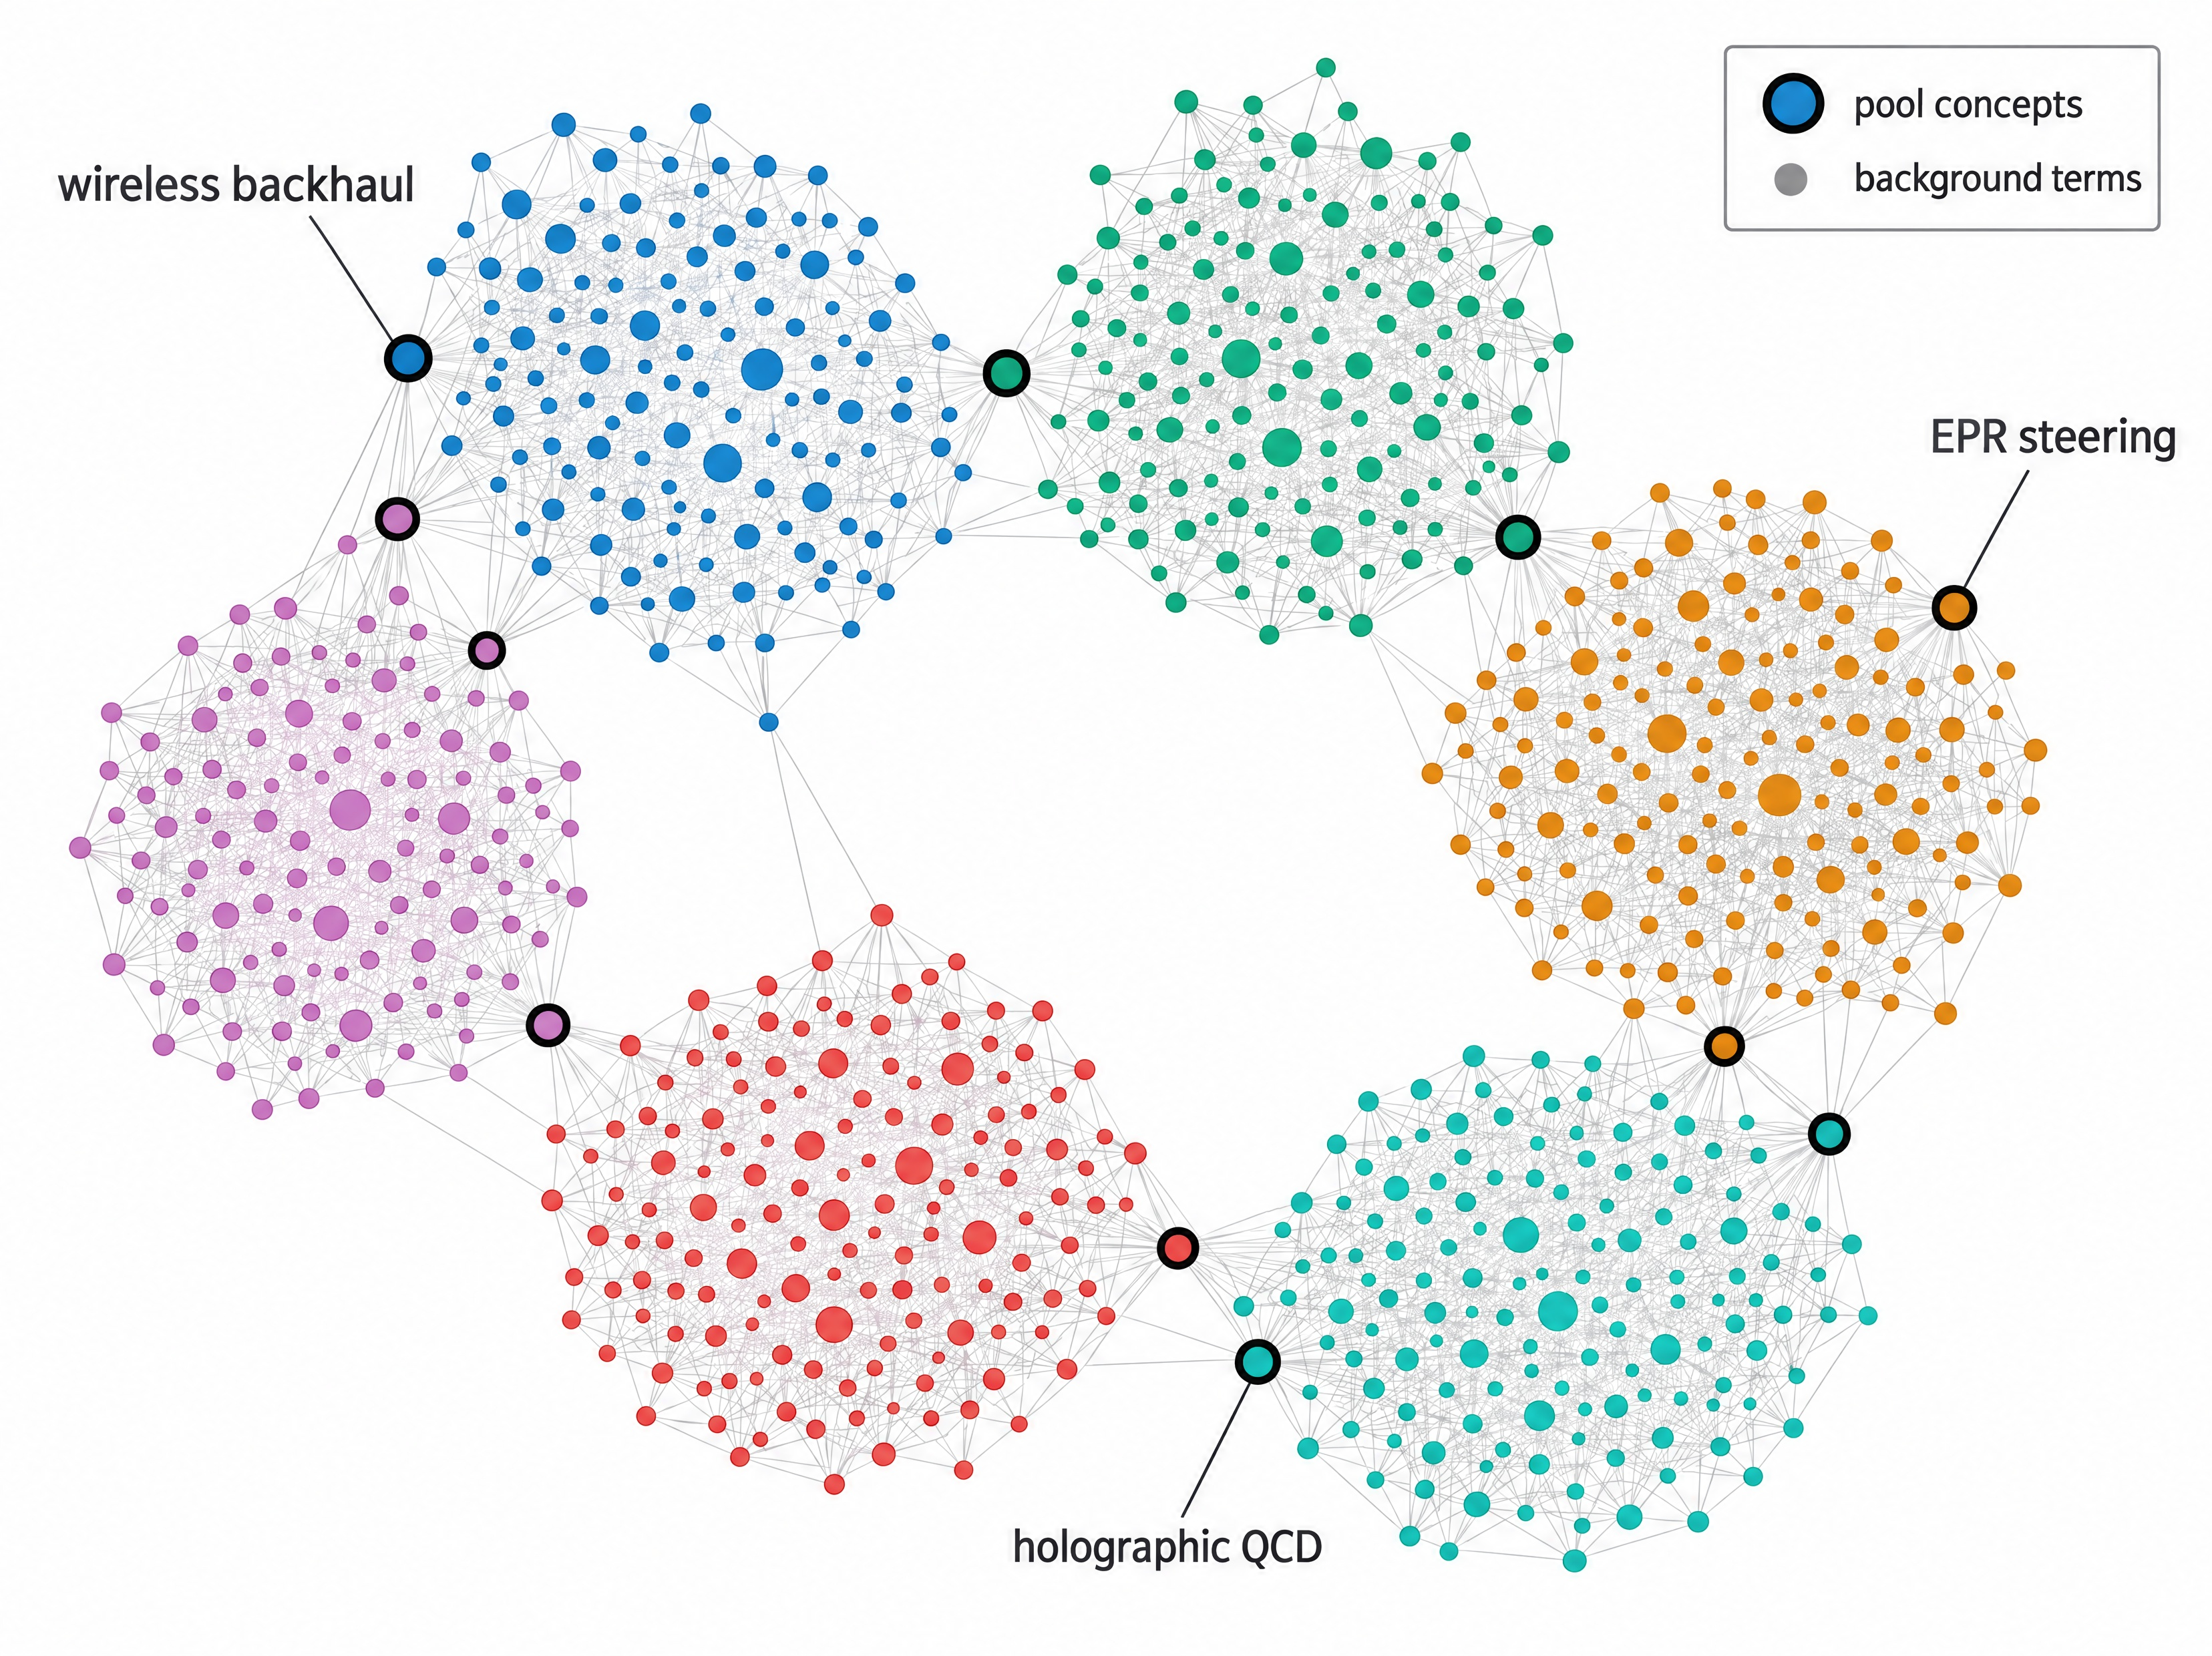
\includegraphics[width=\linewidth,height=0.85\textheight,keepaspectratio]{figures/fig2_v0.jpg}
  \caption{Schematic illustration of the co-word network structure. Nodes represent concept-keyword terms
  and grey edges represent co-occurrence links; node fill colour marks Leiden community
  membership, and larger circles are high-degree hub terms. Background terms (plain nodes) form dense
  communities joined by a few inter-community edges. Pool concepts (bold black rings) sit on the periphery
  of communities, mostly in the gaps between two of them, where they act as bridge or connector nodes; three
  are labelled as examples (\emph{wireless backhaul}, \emph{EPR steering}, \emph{holographic QCD}); their
  placement in the diagram is illustrative and does not reflect their actual network coordinates. The full
  network comprises approximately 27,000 nodes and 84,000 edges; the panel is a schematic rendering
  for readability and does not depict a specific yearly snapshot.}
  \label{fig:network}
\end{figure}

\subsection{Structural precursors of emergence}
\label{sec:rq1method}

\paragraph{Emergence labels.} We defined sustained uptake as a concept-year reaching at least 20 papers per
year and gaining at least 20 percentile points in co-word network strength relative to the focal population.
The focal-population label was declared before outcomes were computed.

\paragraph{Matched event study.} For each concept showing sustained uptake, we matched it to a control concept
from the same first-appearance band and origin field that did not show sustained uptake, using 1:1
nearest-neighbour matching on pre-period network indicators. The standardised mean difference between treated
and control concepts at lags $k = -3$ to $0$ is the event-study estimand. A pooled panel regression of
the binary future-emergence indicator on the closure measure provides a second estimand, reported as the panel
coefficient. Bootstrap confidence intervals ($B = 2{,}000$) and Holm-corrected $p$-values control for multiple
testing. The Screen fold (202 concepts) produced 68 onsets and 26 matched pairs.

\paragraph{Closure measures.} To test whether pre-emergence closure is reducible to neighbourhood turnover
or Burt brokerage, we computed four variants: (a) turnover-residualised closure, obtained by regressing
closure on the new-relation rate, novelty, Baselga beta-similarity, log volume, concept age and Shannon
entropy; (b) persistent-neighbour closure, restricting the closure coefficient to the top-20 neighbours
present in both year $y$ and $y{-}1$; (c) Burt constraint and effective size of the weighted ego
network~\citep{Burt2004}; and (d) cross-community pair excess, defined as the count of partner pairs from
distinct Leiden communities minus the count expected under a strength-decile null.

\subsection{Host-entry grafting}
\label{sec:rq2method}

\paragraph{Host-entry events.} A host-entry event is the first year in which a concept appears in a
non-origin subfield together with at least five co-occurring partner terms. From 4,177 main-arm host entries,
the Screen fold retains 1,544 events across 140 concept clusters after the partner-count filter.

\paragraph{Exposure variable.} Host-vocabulary share is the tag-weighted mean of each partner's pre-entry
publication share in the host subfield, where tag-weighted means that each co-occurrence edge is weighted by
its association strength. The continuous measure is primary because only 1.1\% of partner tags have a host
share above 50\%. Co-transfer is the fraction of partners that were origin companions of the concept in the
five years before entry.

\paragraph{Outcome.} Five-year newcomer uptake: the count of host-subfield papers by author-disjoint newcomers
(authors with no prior concept paper and no co-authorship with concept authors) during the five years after entry.

\paragraph{Model.} Poisson pseudo-maximum-likelihood (PPML) regression~\citep{Silva2006} with
concept-clustered standard errors~\citep{Cameron2015}. Two specifications were pre-registered. The primary
specification includes concept-by-entry-year and host-by-entry-year fixed effects. The co-primary specification
includes concept, entry-year and host fixed effects and was declared for use when the primary drops below 30
concept clusters (which it does on the Held-out fold). Both specifications include co-transfer as a second
regressor.

\paragraph{Held-out fold.} 93 concepts, 1,100 entries; minimum detectable effect (co-primary): IRR per
standard deviation of 1.15. The fold was used during pipeline development (event counts, population sizes and
gating decisions were computed on both folds), so its grafting estimate is a development-set estimate, not a
true held-out confirmation.

\paragraph{MeSH replication.} The same analysis was applied to 191 MeSH concepts. Because the pre-declared
partner-count rule yielded only 192 events, the pre-declared relaxation was triggered, producing 2,171 events
across 160 concept clusters.

\subsection{Post-confirmation decomposition}
\label{sec:decomposition}

After the Held-out and MeSH tests confirmed the host-vocabulary effect, three exploratory decompositions were
pre-specified and frozen before any coefficient was read:

\begin{itemize}
\item \textbf{Extensive versus intensive margins.} A linear probability model for whether any newcomer uptake
occurs (extensive margin), and PPML conditional on uptake having started (intensive margin). Inverse-variance
weighting (IVW) pools estimates across the Screen, Held-out and MeSH folds.

\item \textbf{Host-specific versus generic accessibility.} Generality proxies (tag-weighted normalised subfield
entropy and log block frequency of each partner) are added as controls. The Balassa-index lift
measure~\citep{Balassa1965}, defined as the log ratio of the host-vocabulary share to the partner's baseline
subfield share, is tested as an alternative exposure variable.

\item \textbf{Origin-field dependence.} A Wald test of equality across origin-field groups (Physics and
Astronomy, Computer Science, other).
\end{itemize}

\section{Results}
\label{sec:results}

\subsection{RQ1: Structural precursors of emergence}
\label{sec:rq1}

\subsubsection{Experimental setup}
\label{sec:rq1_setup}

The Screen fold (202 concepts) produced 68 onsets of sustained uptake and 26 matched concept pairs after 1:1
nearest-neighbour matching on pre-period network indicators. The Held-out fold produced 30 onsets and 22
matched pairs; because the Held-out fold's own never-treated pool was too small (33 concepts), 17 of 25 unique
controls were drawn from the Screen fold's never-treated pool, so the Held-out estimator is not fully
control-side independent.

\subsubsection{Results}
\label{sec:rq1_results}

On the Screen fold, concepts that later show sustained uptake have lower general closure in the years before
onset (matched event-study standardised mean difference $= -0.44$, 95\% CI $[-0.81, -0.05]$; panel
coefficient $= -0.66$). The pre-registered positive sign was not observed; the effect runs in the opposite
direction.

\begin{table}[!htbp]
\centering
\caption{Closure on the Held-out fold (development-set estimate). ``Screen panel'' is the panel coefficient on
the Screen fold. ``HO panel'' and ``HO event-study'' are the panel coefficient and matched event-study
standardised mean difference on the Held-out fold. Holm-corrected $p$-values apply to the panel coefficient.}
\label{tab:closure}
\footnotesize
\begin{tabularx}{\linewidth}{X c c c c l}
\toprule
Measure & Screen panel & HO panel & HO event-study [95\% CI] & Holm $p$ & Status \\
\midrule
General closure & $-0.66$ & $-0.39$ & $-0.53\;[-1.20, +0.07]$ & 0.147 & Not confirmed \\
Turnover-resid. & $-0.40$ & $-0.11$ & $-0.27\;[-0.89, +0.30]$ & 0.635 & Not confirmed \\
Persistent-neighbour & $-1.12$ & $-1.07$ & $-0.83\;[-1.71, -0.10]$ & 0.015 & Confirmed \\
Burt constraint & $+0.06$ & $+0.08$ & $+0.11\;[+0.02, +0.19]$ & --- & Positive \\
\bottomrule
\multicolumn{6}{l}{\scriptsize HO = Held-out fold. Holm $p$ tests the panel coefficient.}
\end{tabularx}
\end{table}

Table~\ref{tab:closure} and Figure~\ref{fig:closure} summarise these results. On the Held-out fold (a
development-set estimate; the fold was used in pipeline development), general closure is not significant
(Holm $p = 0.147$). Only persistent-neighbour closure, restricted to top-20 neighbours present in consecutive
years, is significant: the panel coefficient is $-1.07$ (Holm $p = 0.015$) and the matched event-study
standardised mean difference is $-0.83$ (95\% CI $[-1.71, -0.10]$). Burt constraint has the same positive
sign on the Held-out fold (event-study $+0.11$, 95\% CI $[0.02, 0.19]$), indicating that the lower closure
before emergence is not Burt brokerage: concepts that later emerge sit in ego networks that are more
constrained, not less.

The MeSH replication is directional under a sensitivity label (standardised mean difference $D = -0.42$, Holm $p = 0.039$, $n = 29$),
same sign as the main pool, but under the primary label the MeSH effect is null ($D = -0.09$, Holm
$p = 0.677$, $n = 15$).%
\footnote{Code: \url{https://github.com/ai-inventor-papers/ai-invention-8892b7-occupancy-is-not-integration-for-new/tree/fork/run_desxWCcMY1R1/round-2/experiment-4}.}

Structural precursors add no predictive value for whether a concept will later show sustained uptake beyond
frequency, burst, degree and entropy baselines (logistic AUC 0.89 versus 0.88, delta $-0.010$, 95\% CI
$-0.045$ to 0.021).

\begin{figure}[!htbp]
  \centering
  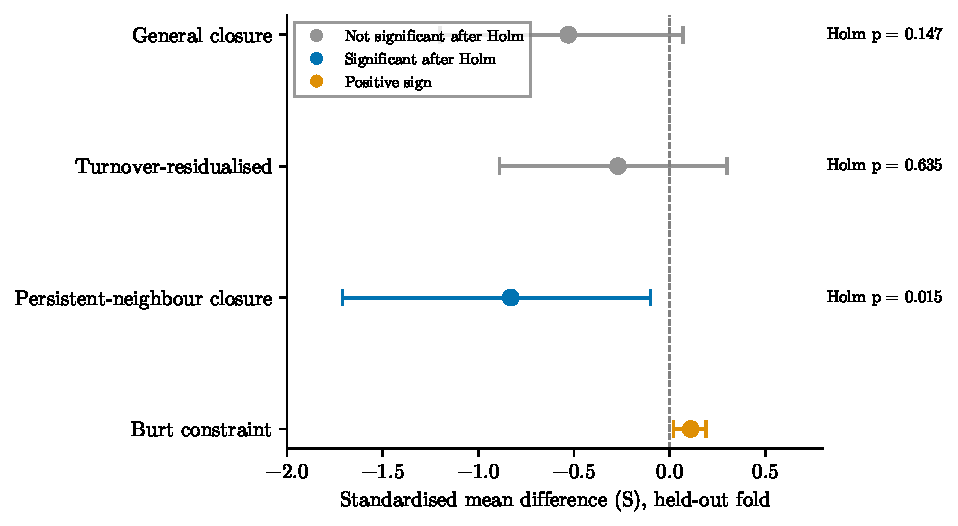
\includegraphics[width=\linewidth,height=0.85\textheight,keepaspectratio]{figures/fig3_v0.pdf}
  \caption{Pre-emergence closure on the held-out fold, by measure type. Each row shows the standardised mean
  difference between concepts that later show sustained uptake and matched controls. Points are estimates
  and horizontal bars are 95\% bootstrap confidence intervals. The dashed vertical line marks no effect,
  and Holm-corrected $p$-values are listed to the right of the first three rows. Only
  persistent-neighbour closure (blue) survives Holm correction (event-study $-0.83$, 95\% CI
  $[-1.71, -0.10]$; panel coefficient $-1.07$, Holm $p = 0.015$). General closure
  (Holm $p = 0.147$) and turnover-residualised closure (Holm $p = 0.635$) are shown in grey: they do not
  survive confirmation, and their intervals cross zero. Burt constraint (orange) is positive ($+0.11$,
  95\% CI $[0.02, 0.19]$), which indicates that emerging concepts sit in more constrained, not more
  brokered, ego networks.}
  \label{fig:closure}
\end{figure}

\subsubsection{Comparison to related work}
\label{sec:rq1_comparison}

The finding that emerging concepts show lower closure among their most stable co-word neighbours is consistent
with the work of \citet{Salatino2018augur}, who found that new topics tend to arise at the intersection of weakly
connected parent areas, and with \citeauthor{Chen2009}'s~\citeyearpar{Chen2009} theory of structural variation
in which transformative work bridges structural holes. It is also consistent with the structural-holes
literature~\citep{Burt2004}: concepts that later emerge connect across Leiden communities, and their
cross-community pair excess is positive. The critical difference is that Burt constraint is higher, not lower.
In Burt's framework, brokerage means low constraint. Here the ego network is more redundant, not less; the
openness is confined to the top of the neighbourhood, while the broader ego network is dense. This pattern is
closer to what \citet{Lin2022} describe as disconnection and discordance enabling new directions in science,
and to \citeauthor{Larson2017}'s~\citeyearpar{Larson2017} finding that weak-tie diffusion in networks is not
guaranteed to carry novel information.

Among Applied Network Science contributions, \citet{Domenico2016} studied knowledge diaspora through
source-sink author flows, and \citet{Cunningham2022} mapped author multidisciplinarity and disciplinary roles
in field-of-study networks, finding that bridge authors between communities can accelerate knowledge transfer.
Our structural analysis complements this by showing that concept-level network openness, not author-level
bridging, precedes emergence. \citet{Fontaine2024} traced the epistemic integration of AI into neuroscience,
showing how vocabulary overlap between fields facilitates absorption, a finding that connects directly to our
host-vocabulary result. \citet{Doonan2019} found that community structure in co-inventor networks affects
time to first citation, paralleling our finding that community position shapes concept uptake.

\subsubsection{Discussion}
\label{sec:rq1_discussion}

The persistent-neighbour closure result indicates that concepts whose top associates do not close into triads
from year to year are more likely to show sustained uptake. General closure is not significant on the Held-out
fold. Burt constraint is positive, meaning the ego network is redundant, not brokered. The picture is of open,
fast-renewing connections among a concept's most strongly associated terms within a dense wider ego network,
rather than brokerage across a structural hole. This is consistent with the finding of \citet{Lin2022} that
disconnection and discordance seed new directions. However, the Held-out fold was used in pipeline development,
so the closure result is a development-set estimate, and the Held-out matching falls back to Screen controls for
17 of 25 unique controls.

\subsection{RQ2: Host-entry grafting}
\label{sec:rq2}

\subsubsection{Experimental setup}
\label{sec:rq2_setup}

The host-entry sample for the Screen fold comprises 1,544 events across 140 concept clusters (co-primary
specification). Entry is predominantly a package: 70\% of partner tags are non-native origin companions, and
only 1.8\% are native grafts (host share above 50\%). The mean host-vocabulary share is 0.043 (SD 0.055). The
Held-out fold has 972 events across 74 concept clusters. The MeSH population has 2,171 events across 160
concept clusters.

\subsubsection{Results}
\label{sec:rq2_results}

\begin{table}[!htbp]
\centering
\caption{Host-entry grafting: pre-registered test. IRR/SD = incidence-rate ratio per one standard deviation
of host-vocabulary share. CT = co-transfer. G = concept clusters. IVW = inverse-variance weighted.}
\label{tab:grafting}
\small
\begin{tabularx}{\linewidth}{l l c c c c c c}
\toprule
Specification & Fold & IRR/SD & 95\% CI & $p$ & CT $p$ & $N$ & $G$ \\
\midrule
Co-primary & Screen & 1.30 & 1.16--1.45 & ${<}\,0.001$ & 0.48 & 1,544 & 140 \\
Co-primary & Held-out & 1.19 & 1.06--1.33 & 0.004 & 0.60 & 972 & 74 \\
Primary (strict FE) & Held-out & 0.98 & 0.70--1.37 & 0.91 & 0.22 & 250 & 30 \\
Co-primary & MeSH & 1.23 & 1.12--1.36 & ${<}\,0.001$ & 0.053 & 2,171 & 160 \\
Primary & MeSH & 1.32 & 1.10--1.60 & 0.004 & 0.46 & 1,004 & 122 \\
Co-primary (IVW) & All three & 1.26 & 1.17--1.36 & ${<}\,0.001$ & --- & --- & --- \\
\bottomrule
\end{tabularx}
\end{table}

Table~\ref{tab:grafting} presents the pre-registered test. On the independent MeSH biomedical population, a
one-standard-deviation increase in host-vocabulary share raises newcomer uptake by 23\% (co-primary IRR 1.23,
95\% CI 1.12 to 1.36, $p < 0.001$; primary IRR 1.32, 95\% CI 1.10 to 1.60, $p = 0.004$; pre-registered
verdict: REPLICATED). The main-arm folds, both used in
pipeline development (event counts, population sizes and gating decisions were computed on both folds before
outcomes were read), give concordant development-set estimates: Screen co-primary IRR 1.30 (95\% CI 1.16 to
1.45); Held-out co-primary IRR 1.19 (95\% CI 1.06 to 1.33, wild-cluster bootstrap $p = 0.012$,
nativeness-permutation $p = 0.026$). Heterogeneity between Screen and Held-out is not significant
($p = 0.25$). The inverse-variance weighted pooled estimate across all three folds is 1.26 (95\% CI 1.17
to 1.36, $I^2 = 0$). Co-transfer is null across all folds and specifications
(Figure~\ref{fig:grafting}).

The fully saturated primary specification on the Held-out fold is inconclusive (IRR 0.98, 95\% CI 0.70 to
1.37) because it retains only 250 of 972 events with 30 concept clusters; this was declared underpowered in
advance (minimum detectable effect IRR 1.30).

\begin{figure}[!htbp]
  \centering
  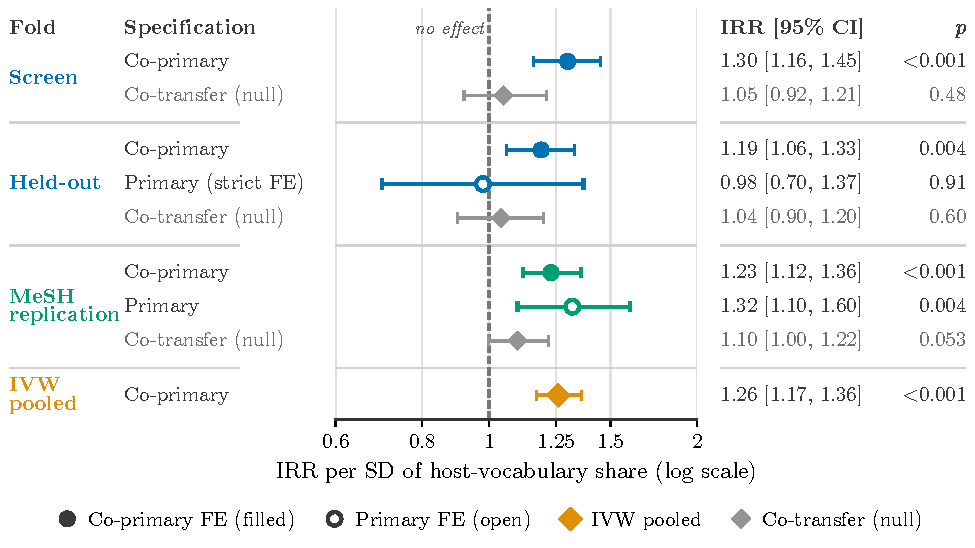
\includegraphics[width=\linewidth,height=0.85\textheight,keepaspectratio]{figures/fig4_v0.pdf}
  \caption{Host-vocabulary effect on five-year newcomer uptake across folds and specifications. Each row gives
  the PPML incidence-rate ratio (IRR) per one standard deviation of host-vocabulary share, on a log axis;
  horizontal bars are 95\% concept-clustered confidence intervals, and the dashed vertical line marks
  IRR $= 1$ (no effect). Filled circles are the co-primary specification (concept, entry-year and host fixed
  effects) and open circles the primary specification with concept$\times$year and host$\times$year fixed
  effects. Blue marks the OpenAlex screen and sealed held-out folds, green the independent MeSH replication,
  and the amber diamond the inverse-variance weighted (IVW) pooled co-primary estimate. The co-primary effect
  is significant on all three folds (screen IRR 1.30 [1.16, 1.45], held-out 1.19 [1.06, 1.33], MeSH 1.23
  [1.12, 1.36]), and the pooled estimate is 1.26 [1.17, 1.36]. The primary specification is inconclusive on
  the held-out fold (IRR 0.98 [0.70, 1.37], 30 clusters, $p = 0.91$) but significant on MeSH (IRR 1.32
  [1.10, 1.60]). Grey diamonds are the co-transfer regressor from the co-primary models. Its intervals
  include 1 on every fold ($p = 0.48$, $0.60$ and $0.053$). The right-hand columns list each estimate with
  its 95\% CI and $p$-value.}
  \label{fig:grafting}
\end{figure}

\paragraph{Robustness.} The co-primary effect holds in 20 of 26 robustness variants on the Screen fold (IRR
range 1.11 to 1.56 among significant rows). All seven pre-specified robustness rows on the Held-out fold are
significant. Nativeness-permutation placebos are centred on 1.0 (co-primary $p = 0.002$ Screen, 0.026
Held-out, 0.010 MeSH). The cluster-robust variance estimator mildly over-rejects at the null (size 10.5\% on
MeSH simulation), so $p$-values should be read alongside the wild-cluster and permutation results.

\subsubsection{Mechanism decomposition}
\label{sec:rq2_mechanism}

\paragraph{Extensive versus intensive margins.} The host-vocabulary effect operates through both the extensive
margin, meaning whether any newcomer uptake starts, and the intensive margin, meaning the count of newcomer
papers given that uptake started. The inverse-variance weighted extensive-margin effect is $+6.4$ percentage
points per standard deviation (95\% CI 4.8 to 8.1, randomisation-$t$ $p < 0.001$), approximately a 13\%
increase relative to the base rate of 51\%. The inverse-variance weighted intensive-margin incidence-rate ratio
per standard deviation is 1.18 (95\% CI 1.10 to 1.27). The extensive share of the total effect is 0.38
(95\% CI 0.21 to 0.55; Figure~\ref{fig:margins}).

\begin{figure}[!htbp]
  \centering
  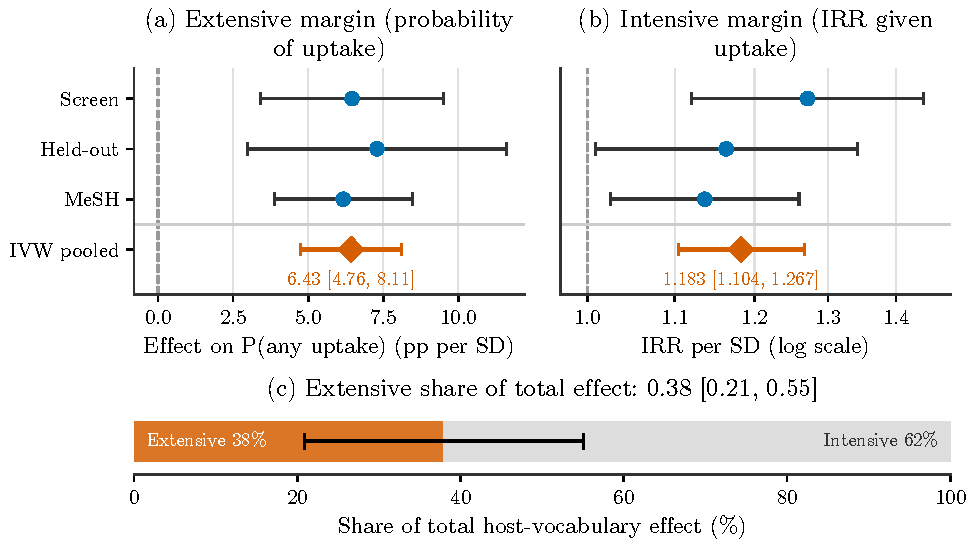
\includegraphics[width=\linewidth,height=0.85\textheight,keepaspectratio]{figures/fig5_v0.pdf}
  \caption{Decomposition of the host-vocabulary effect into extensive and intensive margins across the screen,
  held-out and MeSH folds. Blue circles show per-fold estimates, vermillion diamonds the inverse-variance-weighted
  (IVW) pooled estimate, and horizontal bars 95\% confidence intervals. (a)~Extensive margin:
  linear-probability-model effect of a one-standard-deviation increase in host-vocabulary share on the
  probability of any newcomer uptake, in percentage points per SD (dashed line: no effect). The pooled effect
  is 6.43~pp (95\% CI 4.76 to 8.11). (b)~Intensive margin: PPML incidence-rate ratio per SD conditional on
  uptake, on a log axis (dashed line: IRR $= 1$). The pooled IRR is 1.183 (95\% CI 1.104 to 1.267). All three
  folds are positive on both margins, and every fold interval excludes the null. (c)~Share of the total effect:
  the extensive margin accounts for 38\% (95\% CI 21\% to 55\%, black whisker) and the intensive margin for
  the remaining 62\%.}
  \label{fig:margins}
\end{figure}

\paragraph{Host-specific versus generic accessibility.} Adding generality controls (subfield entropy and log
frequency of entry partners) to the co-primary model retains 97\% of the host-vocabulary coefficient
(inverse-variance weighted retention 0.97, 95\% CI 0.81 to 1.10), and the Balassa-index lift measure is also
significant (inverse-variance weighted IRR per standard deviation 1.34, 95\% CI 1.23 to 1.46). The
host-vocabulary gradient is not reducible to generic concept accessibility. However, within fixed effects the
Balassa-index lift measure has a correlation of 0.997 with the log of the continuous host-vocabulary share,
so the lift leg of this test is weak: the two measures carry nearly the same within-unit information, and the
lift result should be interpreted as confirming the continuous share rather than adding independent evidence
for host-specificity.

\paragraph{No origin-field boundary.} The Wald test for equality of the host-vocabulary effect across
origin-field groups (Physics and Astronomy, Computer Science, other) is null ($p = 0.64$, label-permutation
$p = 0.77$). Physics and Astronomy concepts, whose host-vocabulary coefficient is individually non-significant
(IRR 1.18, 95\% CI 0.93 to 1.50), fall within sampling variation of the other groups.

\subsubsection{Diffusion typology and expansion-before-diffusion ordering}
\label{sec:rq2_typology}

A data-derived typology based on multivariate dynamic time warping of three diversity channels (rarefied
Shannon entropy, Rao-Stirling diversity~\citep{Stirling2007} and active subfield count) yields a stable
two-cluster solution ($k$-medoids, Hennig bootstrap~\citep{Hennig2007} minimum Jaccard 0.86):
\textbf{localised} ($n = 136$, low entropy and few active subfields) and \textbf{broad from the start}
($n = 66$, high entropy from early years). Finer clusterings are unstable ($k = 3$ Jaccard 0.60). The typology
does not separate outcomes better than an entropy-only baseline after residualising on early volume.

Among concepts exhibiting both a co-word-network expansion onset and a disciplinary-diffusion onset, expansion
precedes diffusion in 25 of 26 pooled main-arm cases (proportion 0.96, 95\% CI 0.81 to 1.00, year-shuffle
null 0.62, $p = 0.004$), though only 8.6\% of concepts have both onsets observable. On MeSH, 9 of 13 show
expansion first (not different from the null, $p = 0.43$).

\subsubsection{Adopter-level mechanism}
\label{sec:rq2_adopter}

Adopters, defined as authors who publish a concept paper in the host subfield within the five-year outcome
window, are more likely to have prior corpus exposure to the concept's entry partners than matched non-adopters
from the same host subfield (conditional logistic regression: OR 3.09; prevalence 0.79 versus 0.61; 95\% CI
2.32 to 4.28; 1,013 matched strata, 422 entries, 109 concepts). Exposure to frequency-matched
negative-control concepts is negatively associated (OR 0.62), and the placebo control using partners of a
different concept's entry into the same host is also below 1 (OR 0.72), showing specificity to the concept's
own partners.

Decomposing partners into three vocabulary classes --- FOREIGN (origin vocabulary, host share below 5\%),
ADJACENT (5\% to 30\%) and NATIVE (host vocabulary, above 30\%) --- enrichment follows a gradient: FOREIGN
partners OR 2.88, ADJACENT partners OR 1.91, NATIVE partners OR 1.47. Adopters who pick up a concept in a new
field are most enriched for prior exposure to its origin-vocabulary partners, consistent with the
absorptive-capacity framework~\citep{Cohen1990} in which an individual's ability to recognise and assimilate
external knowledge depends on prior familiarity with that knowledge. This Screen-fold result is not
independently confirmed.

\subsubsection{Representative cases}
\label{sec:rq2_cases}

Four medoid cases from the typology clusters illustrate the host-vocabulary gradient at the concept level
(Figure~\ref{fig:cases}).

\begin{figure}[!htbp]
  \centering
  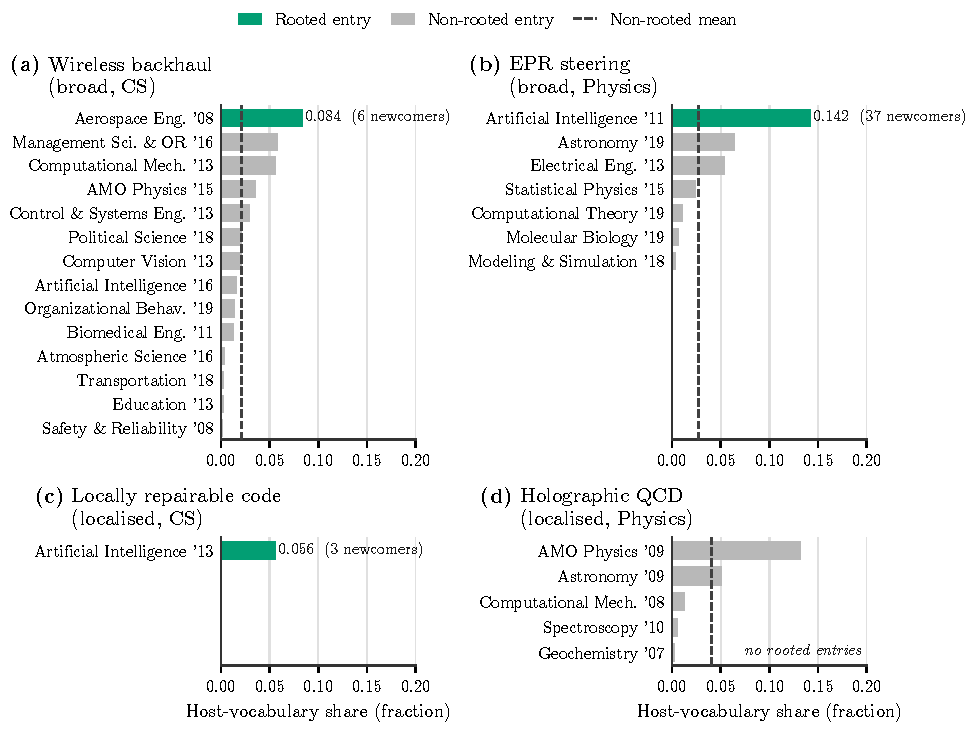
\includegraphics[width=\linewidth,height=0.85\textheight,keepaspectratio]{figures/fig6_v0.pdf}
  \caption{Four representative cases of the host-vocabulary gradient. Each panel shows one concept, and each
  horizontal bar is one of its host entries in the co-primary sample, labelled by host subfield and entry year
  and sorted by host-vocabulary share (x-axis, fraction). Green bars are rooted entries and grey bars are
  non-rooted entries. The dashed line marks the mean share of the non-rooted entries, and rooted bars are
  annotated with their share and number of newcomer papers. (a)~Wireless backhaul (broad, CS): 14 entries, one
  rooted (Aerospace Engineering 2008, share 0.084, 6 newcomers) against a non-rooted mean of 0.021.
  (b)~Einstein--Podolsky--Rosen (EPR) steering (broad, Physics): 7 entries, one rooted (Artificial Intelligence
  2011, 0.142, 37 newcomers; co-transfer 0) against a non-rooted mean of 0.027. (c)~Locally repairable code
  (localised, CS): a single co-primary entry, rooted (0.056, 3 newcomers), so there is no within-concept
  contrast. (d)~Holographic QCD (localised, Physics): 5 entries, none rooted (mean 0.041; three have
  co-transfer 1.0), including an AMO Physics entry at 0.132 that did not take root. In (a) and (b), the rooted
  entry has a higher host-vocabulary share than every non-rooted entry of the same concept. The panels are
  descriptive, so no intervals are drawn.}
  \label{fig:cases}
\end{figure}

\paragraph{Wireless backhaul} (broad type, Computer Science, first appeared 2006). Broad from its first year,
splitting between Computer Networks and Electrical Engineering. By 2022 seven subfields are active. Of 14 host
entries in the co-primary sample, only one is rooted (Aerospace Engineering in 2008, host-vocabulary share
0.084, 6 newcomer papers). The 13 non-rooted entries average a host-vocabulary share of 0.021 and arrive as
origin packages (co-transfer 0.6 to 1.0). Rooted-minus-unrooted host-vocabulary share: $+0.062$.

\paragraph{Einstein--Podolsky--Rosen steering} (broad type, Physics, first appeared 2011). Of 7 co-primary
entries, one is rooted. The rooted entry's host subfield is labelled ``Artificial Intelligence'' in the
OpenAlex subfield taxonomy; this placement arises because OpenAlex files the topic ``Quantum Information
and Cryptography'' under its Artificial Intelligence subfield, which is broader than the colloquial meaning
of AI. The rooted entry has host-vocabulary share 0.142, co-transfer 0,
and 37 newcomer papers. The 6 non-rooted entries average 0.027 with co-transfer at or above 0.55.
Rooted-minus-unrooted: $+0.115$. A broad-type label can hide a concept whose cross-disciplinary integration
rests on a single well-anchored entry.

\paragraph{Locally repairable code} (localised type, Computer Science, first appeared 2013). Stays at 84\% to
96\% in Computer Networks for its life. Has only 1 co-primary entry. The host subfield for this entry is
labelled ``Artificial Intelligence'' in the OpenAlex taxonomy, because OpenAlex files the relevant topic under
its AI subfield, following the same broad assignment noted above.
Host-vocabulary share 0.056, rooted. Demonstrates rooting without broad occupancy.

\paragraph{Holographic QCD} (localised type, Physics, first appeared 2006). Stays at 95\% to 97\% in Nuclear
and High Energy Physics. Its 5 co-primary entries are all non-rooted, averaging 0.041, with three having
co-transfer of 1.0: pure origin packages. No entry is rooted. A locally concentrated concept whose excursions
are packaged imports that do not take root.

\subsubsection{Comparison to related work}
\label{sec:rq2_comparison}

Our host-vocabulary measure is closest to the ideational embeddedness of \citet{Cheng2023}, who found that a
concept's fit with existing traditions raises its yearly article count. Their measure is a global property of
the concept (mean cosine similarity of all its neighbours in a word2vec embedding), whereas ours is
entry-specific: measured at the level of each concept-subfield-year event, with concept and host fixed effects
absorbing concept-level confounds. Co-transfer, the natural competitor, is null. This extends the principle
that relatedness predicts diversification, documented in economic
geography~\citep{Boschma2014, Hidalgo2018}, to the level of individual concept-entry events.

Among Applied Network Science papers, our work engages most directly with the source-sink analysis of
knowledge diaspora by \citet{Domenico2016}, which modelled author flows as diffusion on a bipartite field
network. Our approach replaces author flows with concept-vocabulary composition at the entry point, and finds
that vocabulary, not people, predicts rooting. \citet{Cunningham2022} documented how multidisciplinary authors
occupy bridging positions in field-of-study networks, a role that might facilitate the host-vocabulary
composition we measure. \citet{Fontaine2024} showed that vocabulary overlap between AI and neuroscience
facilitated epistemic integration, and our quantitative test provides the micro-level mechanism consistent
with their macro-level observation. \citet{Holmgren2023} developed multilevel alluvial methods for mapping
change in higher-order networks, related to the alluvial community tracking we use. \citet{Medeuov2021}
appraised discrepancies in semantic networks, finding that endogenous reinforcement within a community is
weak while exogenous diffusion is predictable, consistent with our expansion-before-diffusion ordering.
\citet{Larson2017} showed that weak ties do not guarantee novel information diffusion, complementing our
finding that the vocabulary composition of entry partners, not merely the structural position, predicts rooting.
\citet{Doonan2019} found that co-inventor community structure affects time to first citation, providing
a parallel at the patent level to our concept-uptake results. \citet{Cai2025} examined how knowledge-graph
extraction errors propagate into downstream network analyses, an issue relevant to the OpenAlex concept
assignments on which our co-word network is built.

\subsubsection{Discussion}
\label{sec:rq2_discussion}

The central finding is that a concept's first partners in a new subfield carry information about whether that
concept will subsequently be adopted by newcomer scientists in the host field. The host-vocabulary share
predicts five-year newcomer uptake in a pre-registered design replicated on an independent MeSH biomedical
population (verdict: REPLICATED), with concordant development-set estimates on the main-arm folds.

This result complements the absorptive-capacity framework~\citep{Cohen1990}. At the entry level,
host-vocabulary composition facilitates uptake by newcomers who may not be experts in the concept's origin
field. At the adopter level, the individuals who actually pick up the concept are enriched for prior exposure
to the concept's origin-vocabulary partners (OR 3.09; prevalence 0.79 vs.\ 0.61; Screen fold, not
independently confirmed), consistent with the proposition that recognising external knowledge requires prior
familiarity with it. These two findings operate at different scales: host-native partners lower the barrier for
the field, but the individuals who cross it already speak the origin language.

\subsection{Community roles and bridging}
\label{sec:community}

Leiden community roles (five-seed agreement 97.2\%) partition concepts into four categories: bridge (0.61),
other (0.33), stayer (0.03) and migrant (0.02). Emerging concepts are peripheral or connector nodes in the
Guimera--Amaral cartography~\citep{Guimera2005a} (peripheral 0.49, connector 0.40, kinless 0.10, no hubs).
Lagged roles do not robustly predict host-subfield entry (bridge odds ratio 0.64, 95\% CI 0.38 to 1.08).

Most emerging concepts act as bridges between Leiden communities in the co-word network (early-bridging share
0.70 in the main pool versus 0.59 in MeSH, difference $+0.11$, 95\% CI 0.02 to 0.20), but this bridging role
is common and non-discriminating.

\section{Discussion}
\label{sec:discussion}

\subsection{Null findings and what they bound}

Several pre-registered hypotheses were not supported. Co-transfer, defined as arriving with origin companions,
is null in all specifications and populations, meaning that the composition of entry matters but the
imported-package channel does not. The breadth-prediction screen (does openness predict how many new subfields
a concept will reach?) found no effect beyond growth and level baselines.%
\footnote{Code: \url{https://github.com/ai-inventor-papers/ai-invention-8892b7-occupancy-is-not-integration-for-new/tree/fork/run_desxWCcMY1R1/round-3/experiment-6}.}
The link between pre-emergence closure and later host-entry composition is null (partial correlation 0.025
Screen, 0.053 Held-out, both confidence intervals including zero), meaning that network openness and vocabulary
composition operate independently rather than through a shared mechanism.

\subsection{Limitations}
\label{sec:limitations}

\paragraph{Main-arm folds used in development.} The fold labelled Held-out was used during pipeline
development: event counts, population sizes and gating decisions were computed on both the Screen and Held-out
folds before grafting outcomes were read. Estimates on both main-arm folds are therefore development-set
estimates, not true held-out confirmations. The independent evidence for the host-vocabulary effect comes from
the MeSH replication (verdict: REPLICATED).

\paragraph{Population bias.} The concept pool is dominated by physics, physical-sciences and computer-science
concepts from arXiv. The MeSH population covers only biomedicine-to-biomedicine entries. Generalisation to
social sciences, humanities or engineering is untested.

\paragraph{Primary specification underpowered.} The fully saturated specification with concept-by-year and
host-by-year fixed effects, which absorbs more confounding than the co-primary, is inconclusive on the Held-out
fold (IRR 0.98, 30 clusters). The independent MeSH replication and the development-set estimates rest on the
co-primary specification, which leaves more residual variation.

\paragraph{Single-paper entries.} 87\% of co-primary Screen events involve a single entry-year paper. The
pooled multi-team effect is positive (IRR 1.28, 95\% CI 1.11 to 1.48), but the Held-out alone is underpowered
for this test.

\paragraph{Binary establishment null.} The host-vocabulary share predicts the count of newcomer papers and the
probability that any newcomer uptake occurs, but binary establishment (at least five newcomer papers in at least
three of five years) is null on the Held-out fold ($p = 0.16$). The effect is graded, not threshold-based.

\paragraph{Cluster-robust inference.} The cluster-robust variance estimator rejects 10\% to 11\% of null
shuffles in simulation (target 5\%). Wild-cluster bootstrap and permutation tests give consistent results
(Held-out wild $p = 0.012$, permutation $p = 0.026$), but the standard $p$-values should not be taken at
face value.

\paragraph{Host-specificity caveat.} The Balassa-index lift measure used to test host-specificity has a
within-fixed-effect correlation of 0.997 with the log of the continuous host-vocabulary share. The lift test
confirms the continuous measure rather than providing independent evidence.

\paragraph{Screen-fold adopter evidence.} The adopter-level enrichment (OR 3.09) is Screen-fold only, not
independently confirmed. The design cannot separate absorptive capacity from topical proximity.

\paragraph{Closure Held-out caveats.} The Held-out fold was used in pipeline development, so the closure
result is a development-set estimate. Additionally, the Held-out matching falls back to Screen controls for
17 of 25 unique controls, so the estimator is not fully control-side independent. The MeSH closure result is
directional under the sensitivity label but null under the primary label.

\section{Conclusions}
\label{sec:conclusions}

When a new scientific concept enters a disciplinary subfield, the vocabulary composition of its initial
partners predicts whether newcomer scientists in that field will subsequently adopt it. This host-vocabulary
effect, replicated on 191 independent MeSH biomedical concepts (co-primary IRR 1.23, verdict REPLICATED)
with concordant main-arm development-set estimates (Screen IRR 1.30, Held-out IRR 1.19), is host-specific
--- though the Balassa-index lift leg of this test is near-collinear with the continuous share
(within-fixed-effect $r = 0.997$) --- operates through both the extensive and intensive margins, and does
not vary by the concept's origin field. Co-transfer of origin companions is null.

The complementary structural finding, that persistent-neighbour closure is lower before sustained uptake
(Held-out development-set panel coefficient $-1.07$, Holm $p = 0.015$; event-study standardised mean
difference $-0.83$, 95\% CI $[-1.71, -0.10]$) while Burt constraint is higher, provides the network context:
emerging concepts sit in locally open, fast-renewing neighbourhoods that span multiple communities but are not
brokered in Burt's sense.

These results bear on how knowledge transfer is evaluated and supported. Policies and platforms that facilitate
cross-disciplinary research might benefit from attending to the vocabulary composition of a concept's first
appearance in a new field, rather than only to the mobility of authors who carry it.

Future work should extend the concept pool beyond the physical and computational sciences, test whether the
host-vocabulary gradient holds for social-science and humanities concepts, and design an experiment to separate
absorptive capacity from topical proximity at the adopter level.

\section*{Declarations}

\paragraph{Availability of data and materials.} All data derive from OpenAlex, an open scholarly metadata
index. The concept pool, verified work lists and analysis code are available in the project repository at
\url{https://github.com/ai-inventor-papers/ai-invention-8892b7-occupancy-is-not-integration-for-new}.

\paragraph{Competing interests.} The author declares no competing interests.

\paragraph{Funding.} Not applicable.

\paragraph{Authors' contributions.} Not applicable.

\bibliographystyle{plainnat}
\bibliography{references}

\end{document}
